\subsection{Autonomous comparison with a refreshed route table}
\label{sec:strong-autonomous}
We compare the composable route table and the contract verifier on 60 new state pairs (120 synthetic tasks). Three repetitions per backend give 720 runs with the same hosted Qwen3.8-Flash alias. The design matches tools, authorization, confirmation and recovery across backends. A business checkpoint schedules changes independently of raw read requests. It includes return of a preferred route, a change after a committed effect, and loss of all authorized continuations. A separate condition updates the evidence version while keeping the same route admissible. Appendix~\ref{sec:autonomous-protocol} describes the protocol.

\begin{table*}[t]
\centering
\small
\begin{tabular}{@{}lrrrrrrr@{}}
\toprule
Backend & Correct & Excess & Recoveries & Raw fields & Tool calls & Model calls & Approvals\\
\midrule
Refreshed route table & 360/360 & 0 & 177/177 & 630 & 5,000 & 5,356 & 420\\
Versioned contracts & 359/360 & 0 & 265/265 & 629 & 5,125 & 5,490 & 419\\
\bottomrule
\end{tabular}
\caption{Autonomous comparison on Qwen3.8-Flash. Correct outcomes include 60 expected safe stops per arm. Recovery is conditional on a blocked read. All 177 matched runs blocked by both backends achieved the correct outcome in both arms.}
\label{tab:strong-autonomous}
\end{table*}

Both backends recorded zero excess field releases and zero exact-value disclosure in visible model text. The one incorrect outcome was a contract-arm run that changed the pickup point then received an HTTP 400 before booking. In 90 matched runs with unchanged route eligibility and an updated evidence version, the contract arm recorded 85 evidence-expiration denials. The two arms used 1,219 and 1,423 tools respectively. Over all tasks the contract-minus-table paired mean difference is 0.347 tool calls, with a 95\% task-pair bootstrap interval of $[-0.308,0.961]$. These observations identify a recovery cost when version binding is stricter than current eligibility. They show no incremental reduction in excess releases on this suite.

\paragraph{Replication with Qwen4-Max.}
We repeat all 720 assignments with the same tools, task pairs, seeds and budgets. Both arms produce 360/360 correct outcomes, zero excess field releases and zero visible exact-value disclosures. The table recovers after all 180 read blocks. The contract arm recovers after all 270, including 90 denials where evidence versions changed and the route remained eligible. Total tool calls are 10,867 and 10,885 respectively. Through the terminal business outcome, the counts are 3,810 and 4,170. All 360 additional pre-closure calls occur in the 90 version-only runs. Another 7,057 and 6,715 calls occur after workflow closure (Figure~\ref{fig:strong-stage-cost}). Normal final replies occur in 121 and 122 runs; all 45 gateway interruptions follow a correct business outcome. The execution ledger and the dialogue endpoint measure distinct aspects of agent performance.

\begin{figure*}[t]
\centering
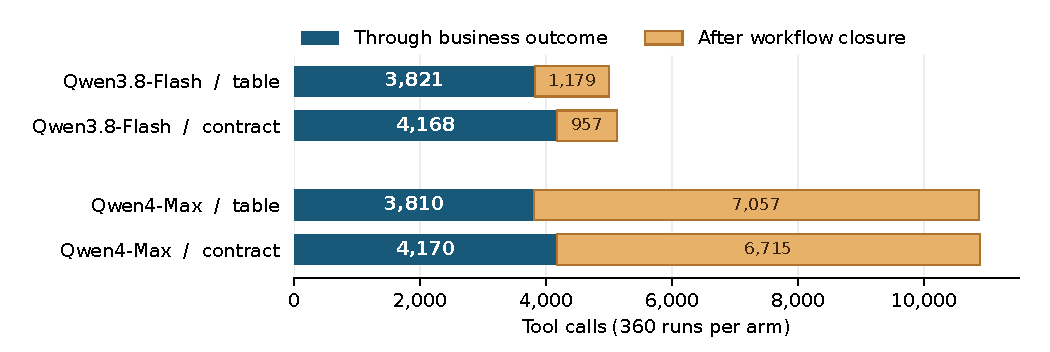
\includegraphics[width=\textwidth]{figures/strong-call-stages.pdf}
\caption{Tool calls through the business outcome and after workflow closure for the strong-baseline comparison. The shared original tool protocol remains in force for both models. The after-closure segment accounts for most of the Qwen4-Max aggregate cost.}
\label{fig:strong-stage-cost}
\end{figure*}

\subsection{Rule maintenance and audit}
We add three business rules covering changed bank details, cross-region pickup moves and restricted-site bookings. Both backends use three authored rule declarations. The table names three reusable recipe fragments. The contract configuration names four tools. The table additionally regenerates four existing and four new recipe entries. Both share the same generated business operation catalog. Both pass 36 policy fixtures, retain behavior on 12 old paths per backend, and detect all 15 injected faults per backend. Faults cover missing rules, selector changes, condition reversal, wrong field binding and missing prerequisites. The results measure configuration artifacts and regression coverage. Human authoring time and natural misconfiguration rates remain open.

Each backend emits enough information to reconstruct eight curated decisions after we add a shared structured log. It records rule identifiers, requested fields, prerequisites, and current and prepared evidence versions. Native contract logs include successful reads, while neither native interface carries the rule identifier in these cases. A separate reconciliation of approved rules and deployed configuration pinpoints all 15 faults per backend. The audit result therefore supports explicit instrumentation and configuration reconciliation for either implementation.

\subsection{Exploratory second-model compatibility}
A matched pilot runs six strong-baseline tasks with both backends using Qwen4-Max and compares the corresponding Qwen3.8-Flash records under the same tool protocol and budgets. Each model achieves 12/12 correct business outcomes and zero excess field releases. Qwen4-Max produces a normal final reply in 5/12 runs, compared with 12/12 for Qwen3.8-Flash. Tool calls rise from 158 to 340, with after-completion calls rising from 22 to 204. In this pilot the extra calls arise after the business outcome is settled. The strong-backend replication is reported in Section~\ref{sec:strong-autonomous}. Sections~\ref{sec:airgap-adaptation} and~\ref{sec:factorial} report the remaining replications. Token limits and finishing behavior are tracked separately from business completion.

In a separate matched diagnostic on six other tasks, we change only the response to a tool call after the workflow is closed. Both feedback formats achieve 12/12 correct business outcomes and zero excess releases. Explicit closure feedback increases normal final replies from 4/12 to 12/12 and cuts after-closure calls from 225 to 8. Calls before closure total 136 in each condition. This diagnostic isolates a tool-protocol effect on observed cost and is recorded separately from the full replication.
